
	En el punto anterior se describió el algoritmo de Kalman. En dicho algoritmo hay una fase de inicialización de la estimación. En este punto intentaremos exponer las variantes que se presentan a la hora de inicializar. Por ejemplo podemos inicializar en un valor correcto, con una varianza pequeña, en cuyo caso la estimación convergerá mas rapido. Otro caso extremo es cuando inicializamos con un valor incorrecto, tambien con varianza pequeña, en cuyo caso la estimación convergerá en forma mucho mas lenta. La idea de este punto es explorar las distintas variantes de este tema. Para cada caso presentaremos gráficos de la estimación de la trayectoria, de evolucion de los errores, y de la autocorrelación de las innovaciones.
	
	\subsection{Caso 1}
	
		Para el primer caso, se tiene un error en la estimación del estado inicial pequeño, pero una varianza grande. En este caso el algoritmo convergerá rapidamente a la trayectoria real. El resultado puede verse en la figura \ref{fig:ej3a}.
	
		\begin{figure}[H]
			\centering
			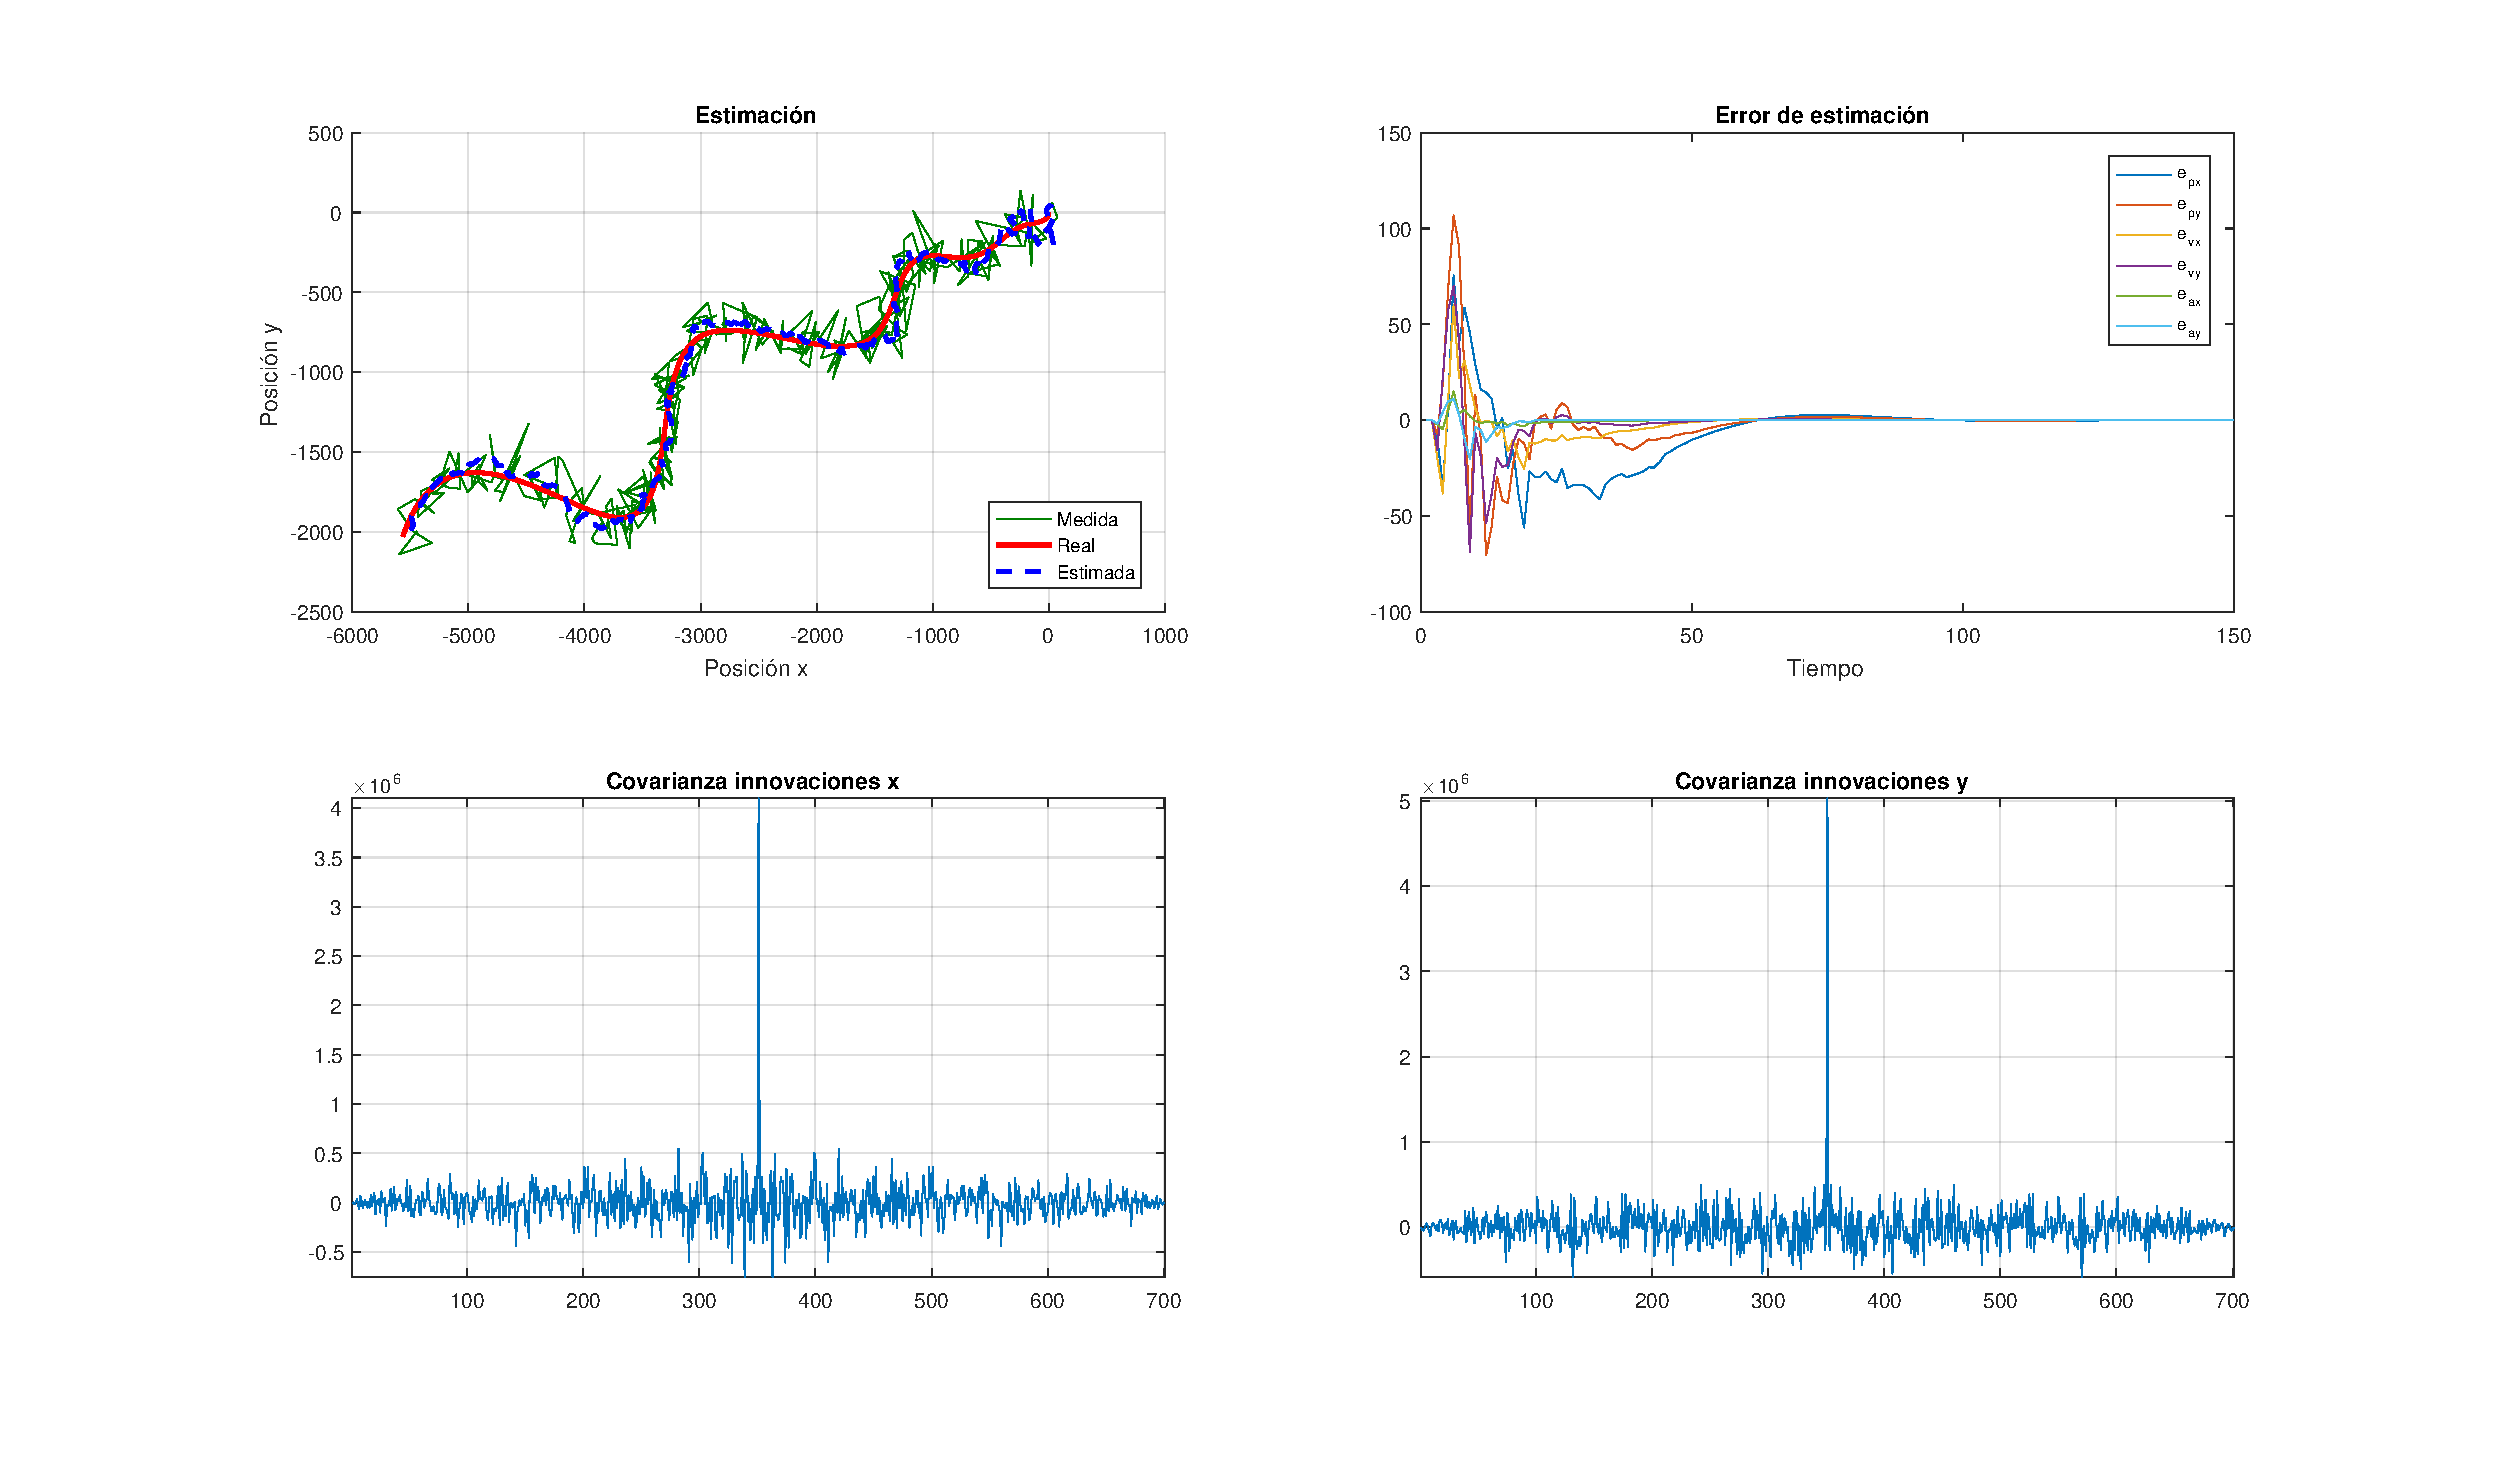
\includegraphics[width=1.0\textwidth,keepaspectratio]{Figuras/graf_ej3a.pdf}
			\caption{Caso 1}
			\label{fig:ej3a}
		\end{figure}
	
	\subsection{Caso 2}
	
	En este segundo caso se tiene un error en el estado inicial grande, pero al ser la varianza grande, el algoritmo sabe que se trata de un valor poco confiable, y no tarda demasiado en corregir la estimación de la trayectoria. El resultado puede verse en la figura \ref{fig:ej3b}.
		
		\begin{figure}[H]
			\centering
			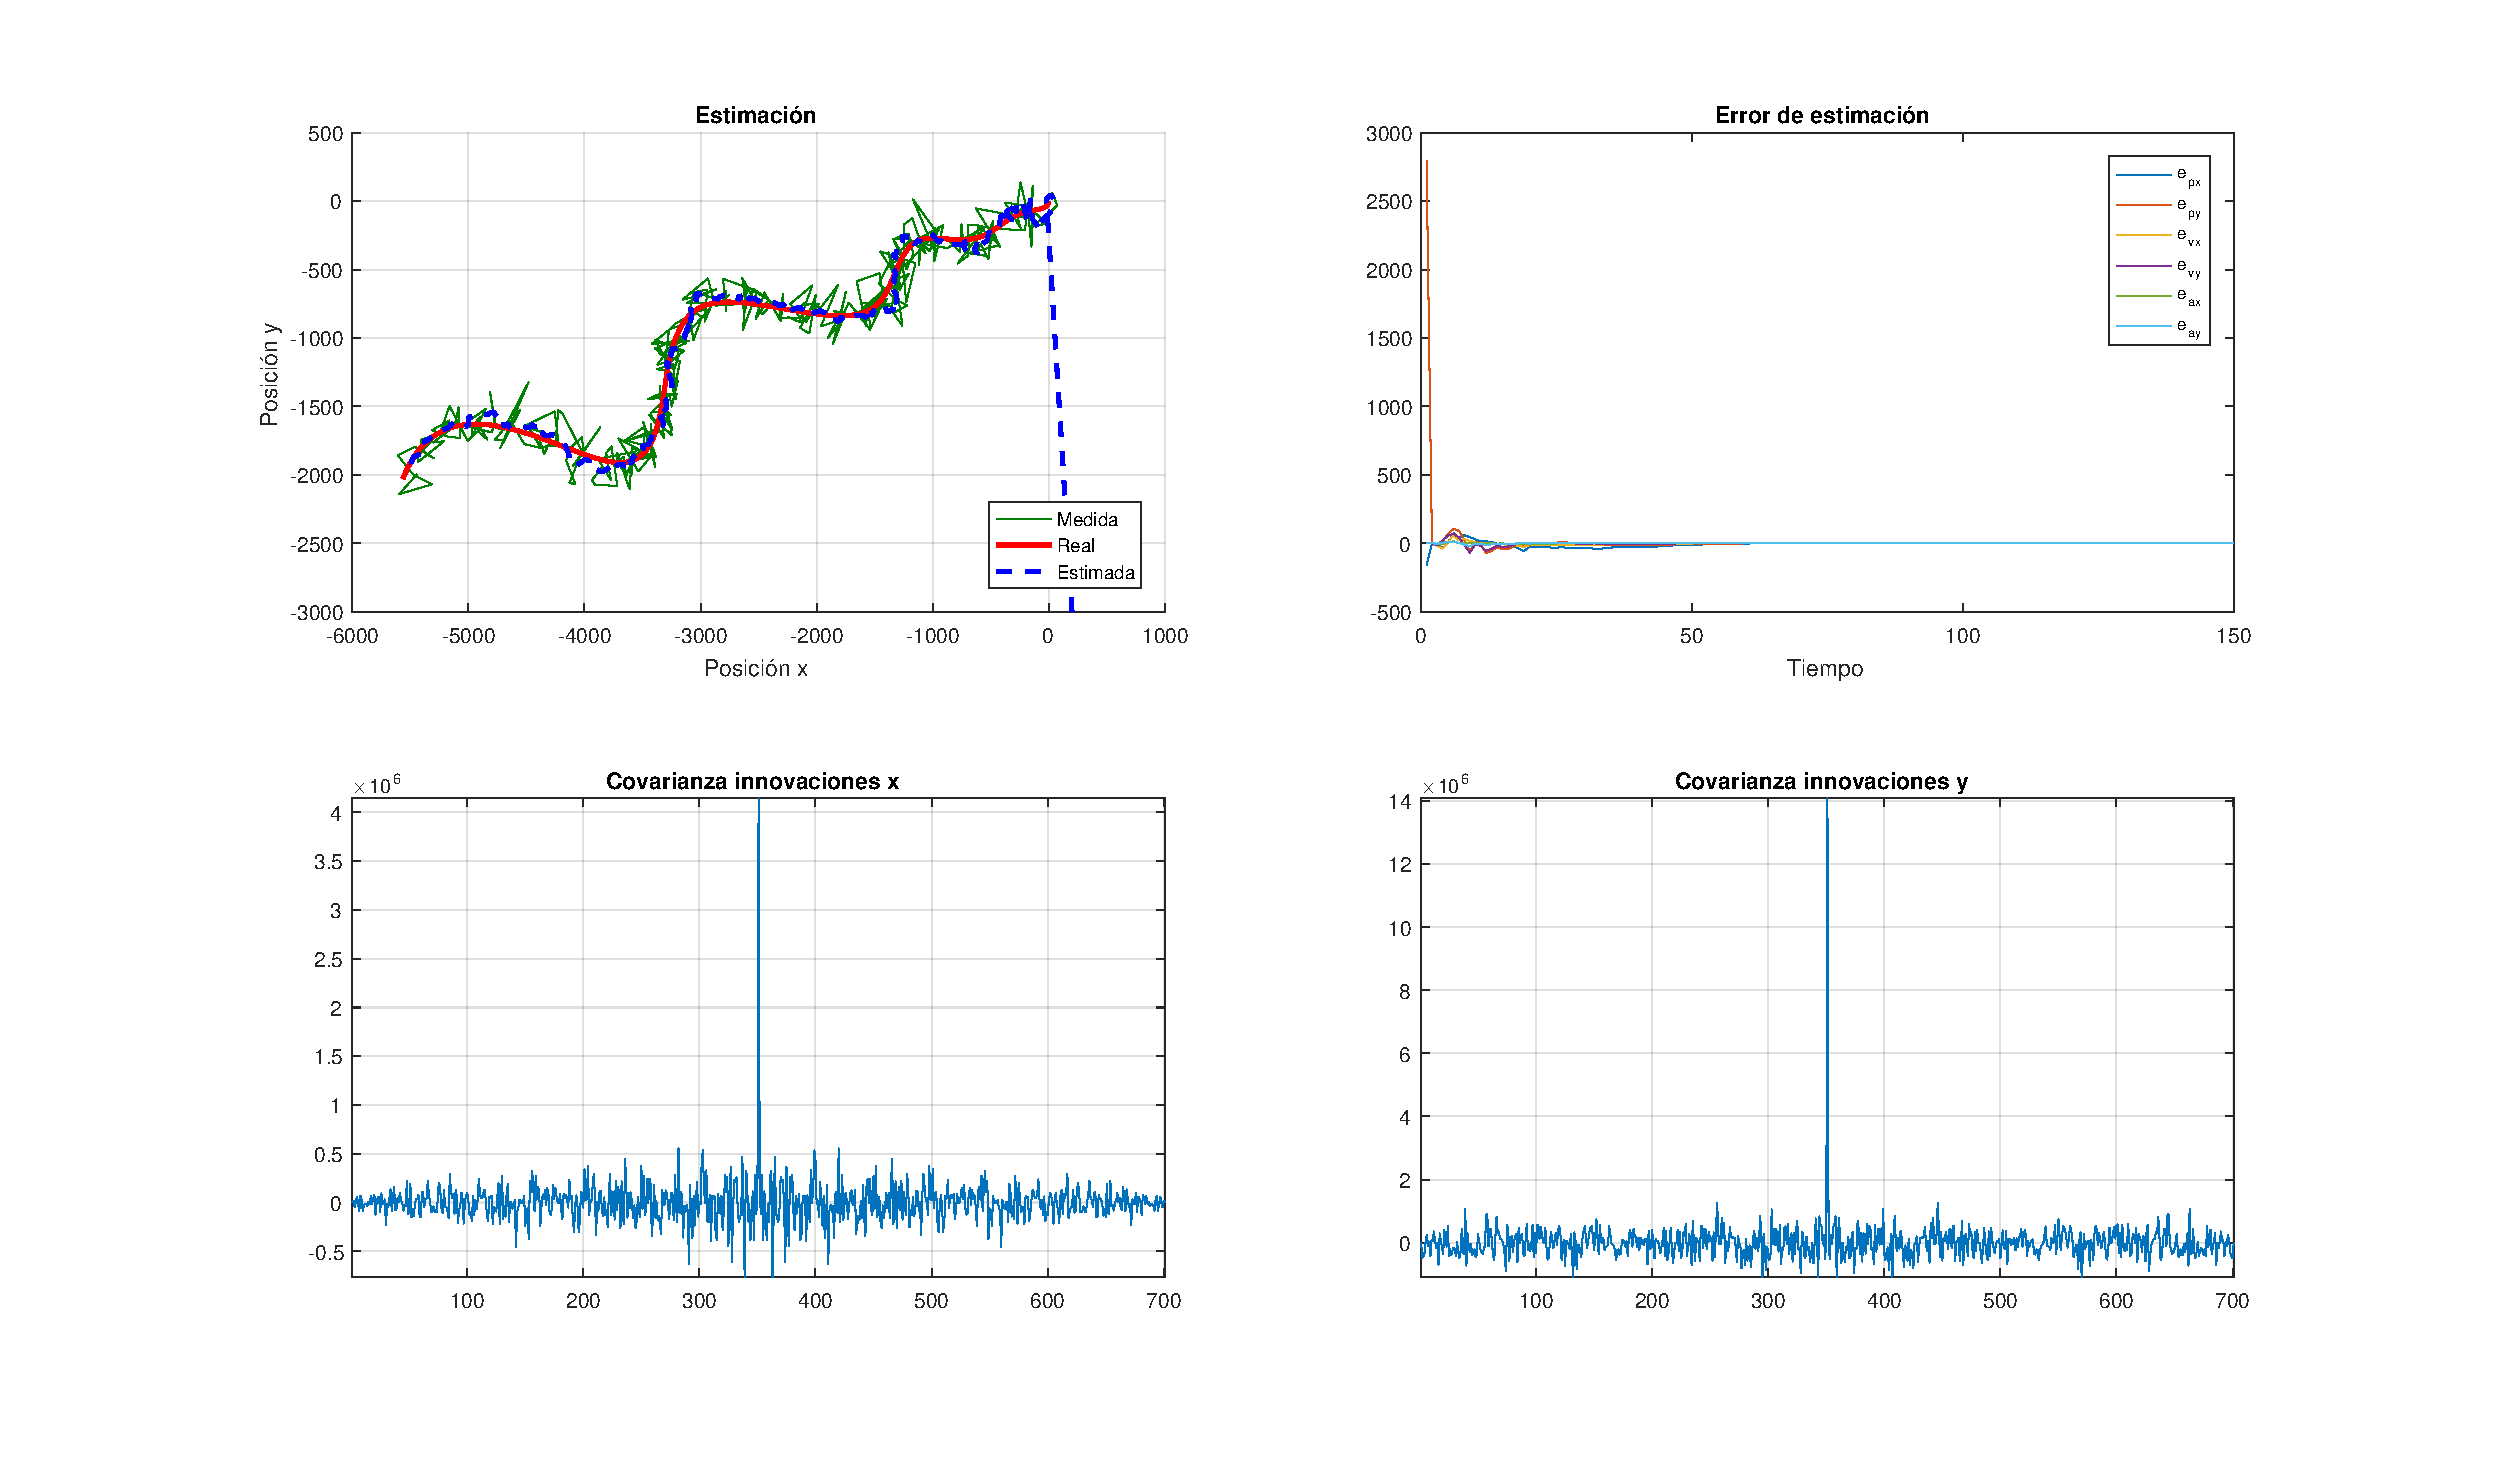
\includegraphics[width=1.0\textwidth,keepaspectratio]{Figuras/graf_ej3b.pdf}
			\caption{Caso 2}
			\label{fig:ej3b}
		\end{figure}
	
	\subsection{Caso 3}
	
	En este tercer caso el error de la estimacion del estado inicial es pequeño, pero a diferencia del primer caso la varianza es grande. Al ser la varianza grande, el algoritmo le dará menos confianza al dato del valor inicial y tardará mas en converger que en el primer caso. El resultado puede verse en la figura \ref{fig:ej3c}.
	
		\begin{figure}[H]
			\centering
			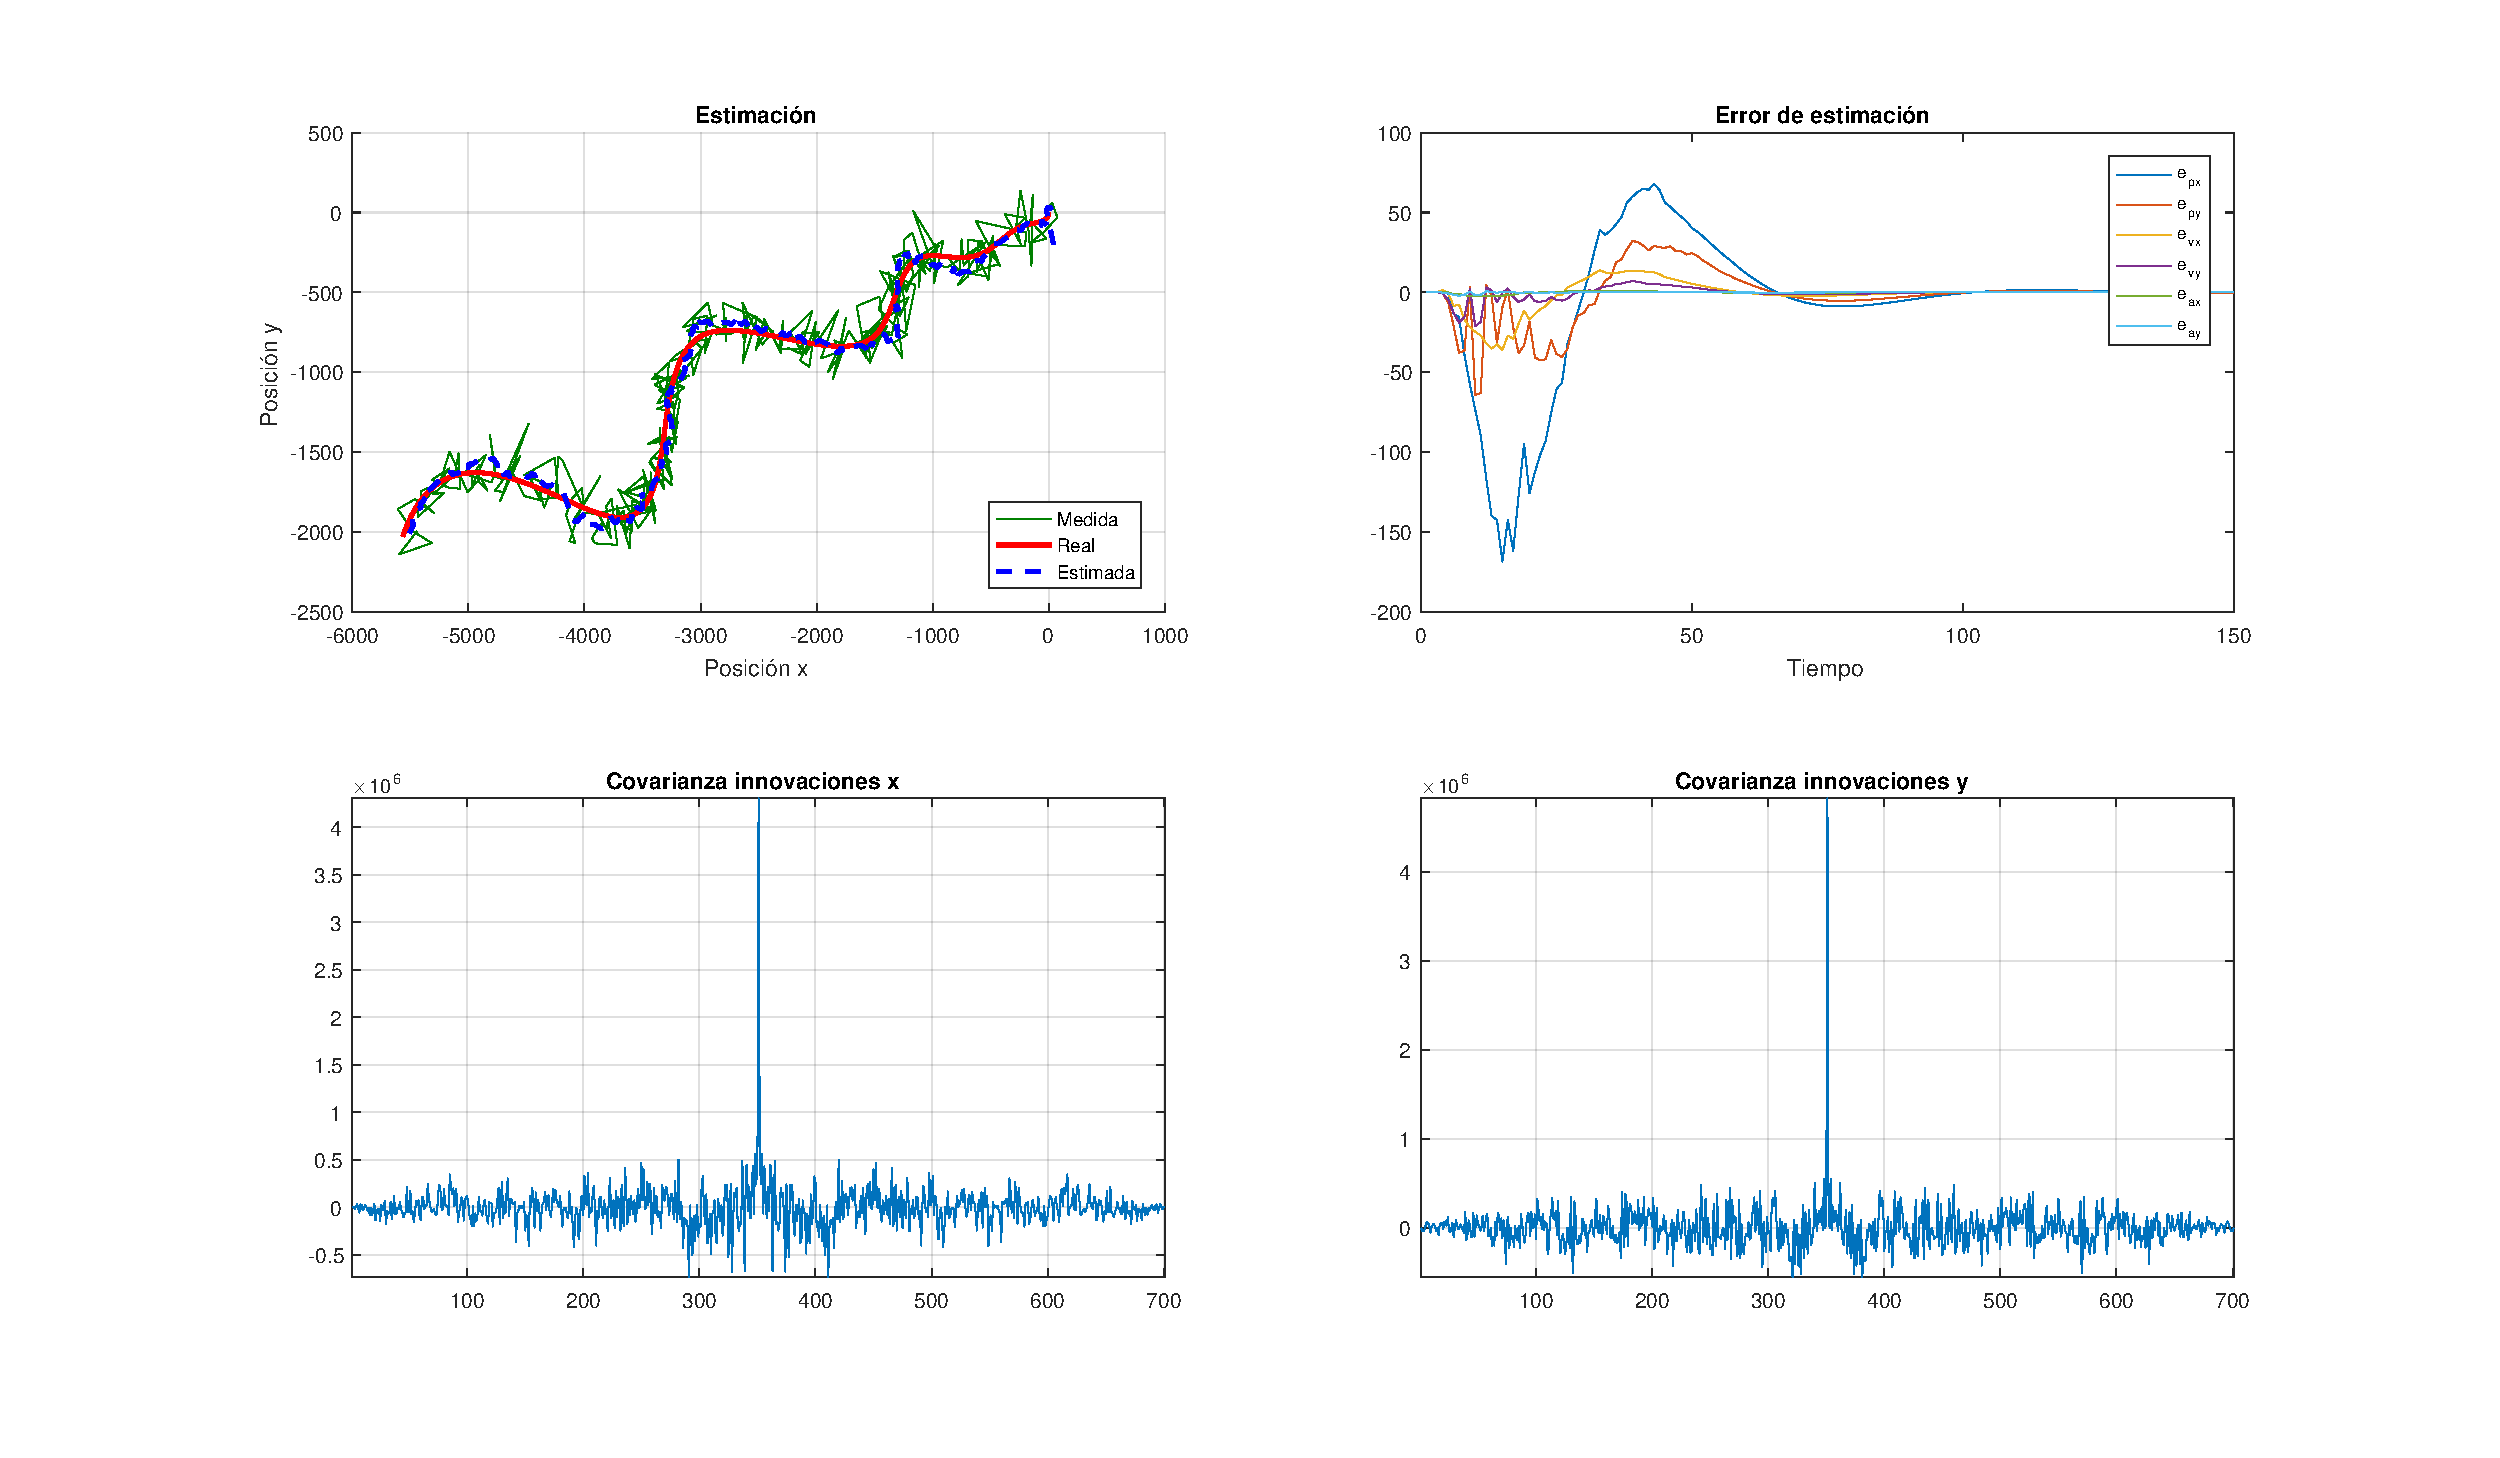
\includegraphics[width=1.0\textwidth,keepaspectratio]{Figuras/graf_ej3c.pdf}
			\caption{Caso 3}
			\label{fig:ej3c}
		\end{figure}
	
	\subsection{Caso 4}
	
	Este ultimo caso es la peor condición, dado a que se tranta de un error en el estado inicial grande, con una varianza pequeña. Es decir  se está informando al algoritmo con un estado inicial incorrecto, pero además, se le esta informando de que es muy confiable. El resultado puede verse en la figura \ref{fig:ej3d}.
	
		\begin{figure}[H]
			\centering
			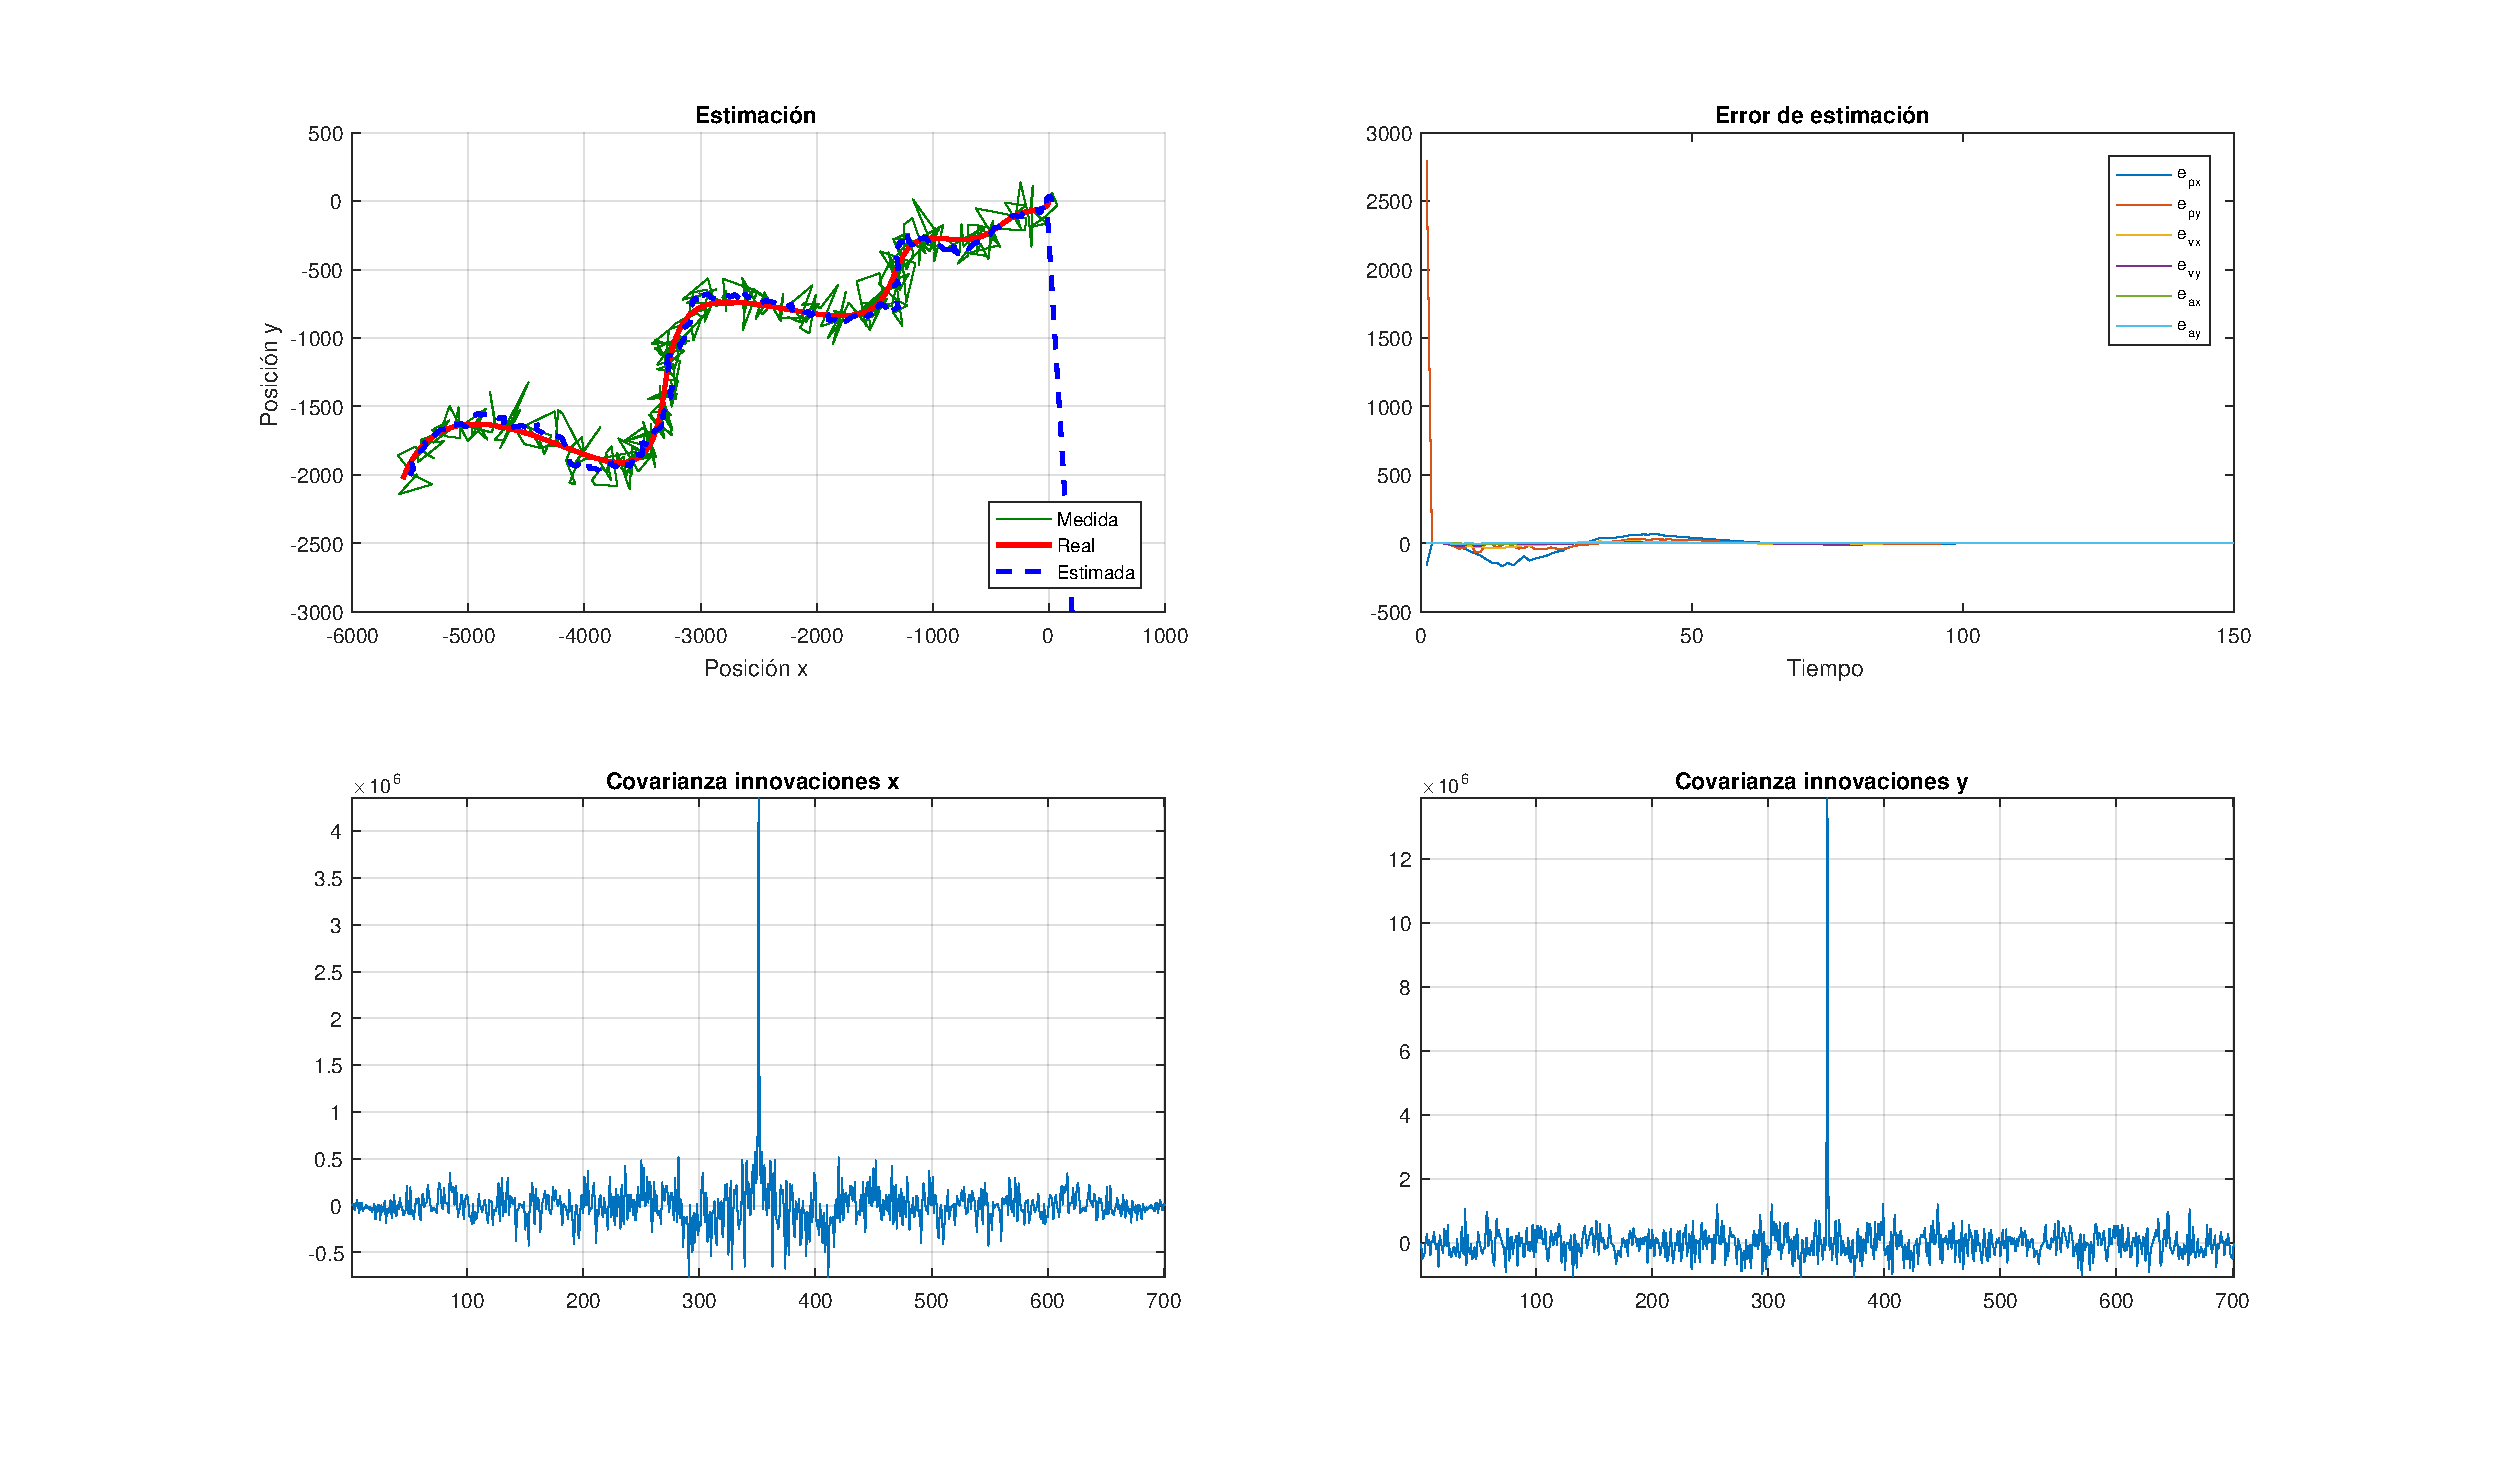
\includegraphics[width=1.0\textwidth,keepaspectratio]{Figuras/graf_ej3d.pdf}
			\caption{Caso 4}
			\label{fig:ej3d}
		\end{figure}
		
	\subsection{Script}
	
		A continuacion presentamos el script de esta sección. Basicamente realiza lo mismo que el punto anterior, pero para distintas condiciones iniciales.

	%\lstinputlisting[]{../Octave/EJ3.m}
	
